\documentclass[11pt]{article}
\usepackage{graphicx}
\usepackage{amssymb}
\usepackage{amsmath}
\usepackage[backend=bibtex,style=ieee,bibencoding=ascii,sorting=none]{biblatex}
\usepackage{fancyhdr}
\usepackage{geometry}
\usepackage[export]{adjustbox}
\usepackage{subcaption}

\geometry{left=1in, right=1in, top=1in}
\pagestyle{fancy}
\fancyhf{}
\fancyhead[L]{Carlos Martinez-Villar}
\fancyhead[C]{STAT 9100}
\fancyhead[R]{Final Project Report}
\title{Final Project Report\\STAT 9100 - Statistical Learning with Networks}
\author{Carlos Martinez-Villar}
\date{\today}
\addbibresource{refs}

\begin{document}
	%\maketitle
	%%%%%%%%%%%%%%%%%%%%%%%%%%%%%%
	% INTRODUCTION
	%%%%%%%%%%%%%%%%%%%%%%%%%%%%%%
	\section{Introduction}
	The present report discusses Hopfield networks (HNs) and some of their properties in relation to the subjects presented throughout this semester as a network that can learn.
	The report is organized as follows: the second section includes a somewhat detailed description of the Hopfield model. 
	Subsections therein describe the equations and rules that were needed to implement a simple version of this model and make it work.
	The last two of these subsections include a broader discussion of these models' context with analogies to statistical physics and the Ising model. 
	The third section includes results of the implementation, and a brief discussion of the shortcomings found. 
	
	%%%%%%%%%%%%%%%%%%%%%%%%%%%%%%
	% MODEL
	%%%%%%%%%%%%%%%%%%%%%%%%%%%%%%
%	\cite{hebb2005organization}
%	\cite{mackay2003information}

	\section{Hopfield's Model and Methods}
	
	The bulk of the method used here was proposed early on by Hopfield in \cite{hopfield1982neural}  and \cite{hopfield1984neurons} as a system consisting of individual nodes that–despite being very simple individually–showed collective properties with representational power. This collective representational power was higher than the individual representational power of the constituent elements, so the system was capable of storing a system-wide state based on the states of individual elements. 
	
	This relation between individual and collective states was analogous–as Hopfield noted–to physical systems where "interactions among a large number of elementary components yield collective phenomena such as stable magnetic orientations [...] or vortex patterns in fluid flow". Since his goal was to find a comparable collective computational phenomenon that could arise from a set of neurons, he considered that finding a stable system state (i.e.: an attractor) must be akin to categorizing a general concept or \textit{gestalt}, and/or correctly storing and retrieving a memory.
	
	Hopfield initially proposed as a content-adressable memory which is–basically–any storage system that can find data from a partially matching search term given to it. Thus the solution given in the original paper was presented as a network that could (i) learn a pattern and (ii) converge to a closest pattern when shown a partial pattern.

	\subsection{Model Specification} 
	Haykin \cite{haykin} describes HNs, within the grand scheme of neural networks, as a neurodynamic recurrent network with a global feedback system. This is quite different from neural networks commonly used in deep learning \cite{deeplearning2015} which have a clear direction forward and backward direction.
	The feedback property can be appreciated through the diagrams in figure \ref{fig:net} which shows a Hopfield network with 4 neurons. Figure \ref{fig:netcircuit} shows the commonly used circuit diagram for a Hopfield network, and figure \ref{fig:netgraph} shows an equivalent graph similar to those studied throughout the semester. The latter diagram is equivalent to the former if we assume that a single edge in figure \ref{fig:netgraph} is equivalent to two directed edges in either direction in figure \ref{fig:netcircuit}. This can be written as $w_{ij} = w_{ji}$ where $w_{ij}$ is the connection strength between nodes (neurons) $i$ and $j$. 


	\subsubsection{Update Rule}
	The original model introduced by Hopfield in \cite{hopfield1982neural} considered binary states for each neuron. Let $x_j \in \{ -1, 1 \}$ be the state of a node $j$ for $j=1,\ldots ,N$ in a network of $N$ neurons. Each node will change its state according to an input defined by the nodes connected to it (its neighborhood). If a set of interaction weights $W$ are known, then we can determine the individual state of a node $x_j$ by 
		
	\begin{equation} \label{eq:nodeupdate}
		x_j = \begin{cases}
			 -1  & \text{if } \sum^{}_{i \neq j} x_i W_{ij}  < -b_j \\
			1  & \text{if } \sum^{}_{i \neq j} x_i W_{ij} \ge -b_j
		\end{cases}
	\end{equation}
	
	so that each node will set its state to -1 or 1 depending upon whether the sum of its inputs coming from all other nodes $i$ adds up to a number below or above a threshold.
	
%	\subsubsection{Updating Edge Weights Between Nodes}
%	In a system with $N$ neurons, the term $W$ in equation \ref{eq:nodeupdate} can be taken to be an $N\times N$ matrix representing the connections between each of these neurons (nodes) in the system described in the following section.
%	
%	\begin{equation}
%		w_{ij} 
%	\end{equation}
	
	\subsubsection{Storing a Pattern}
	If we would like the network to recall a pattern, one way to set up the weights is to set each $w_{ij}$ between any two nodes in the array of weights (edges) $W_{ij}$ according to the agreement between nodes. This agreement or disagreement is represented by positive or negative numbers as
	\begin{equation}
	\begin{cases}
		W_{ij} > 0 \ \text{between nodes $i$ and $j$ in the same state}\\
		W_{ij} < 0 \ \text{otherwise}
	\end{cases}
	\end{equation}
	
	Given this condition, and provided with a pattern we wish to recover, we can let the network adjust and find an appropriate set of weights to recall that state. The idea here is that, once the matrix $W$ is set, we can feed the network anything and expect it to recover the pattern that was used to set $W$.  

	\subsubsection{Storing Multiple Patterns}
	We can call a set of multiple patterns memories. One way to store multiple such memories in a network is to follow Hopfield's original prescription of letting the weights change by $\Delta W_{ij}$ so that this delta is the average co-activation between nodes over the set of memories. Let $X$ be a vector of size $N$ representing the state of our network of $N$ neurons. We can have our memories be the set of states  $\{ X^{(1)}, \ldots, X^{(M)} \}$. Then
	\begin{equation}
		W = \frac{1}{M} \sum^{M}_{s=1} x^{(s)}_i x_j^{(s)}, \ \ i\neq j
	\end{equation}
	Our typical adjacency matrix then becomes this co-activaction array with each $W_{ij}$ being the \textit{average co-activation between nodes} $i$ and $j$. Since we are multiplying each node with each other for each state, this is previous equation is the mean of the outer product of the state vectors $X^{(s)}$.
	
	
	\subsection{The Idea of Energy in Hopfield Networks}
	The most interesting concept in HNs, and perhaps the one that pertains the subject of the course the most is the concept of Hopfield energy. 
	
	\begin{equation}
		E = \sum^{}_{i \neq j}= - \sum^{}_{i < j} s_i s_j w_{ij} - \sum^{}_{i} s_i b_i
	\end{equation}	
	\begin{equation}
		E = -\mathbf{s}^T W\mathbf{s} - \mathbf{s}^T b	
	\end{equation}
	
	\subsubsection{Relation to Gradient Descent}
	Gradient descent–or rather stochastic gradient descent–is today the most common method for optimizing neural networks [citation needed]. 
	
	\begin{equation}
		\frac{\partial E}{\partial x_j} = 
	\end{equation}
	\begin{equation}
		\frac{\partial x_j}{\partial t} = 
	\end{equation}
	\begin{equation}
		\frac{\partial E}{\partial w_{ij}} = 
	\end{equation}
	
	More interestingly, this derivative of $\frac{d x_j}{dt}$ agrees with the update rule equation prescribed iby \ref{eq:nodeupdate}, making sense of what a node does when taking a step in the energy surface. 	
	
	\subsubsection{Settling to an Energy Minimum}
	
	
	%%%%%%%%%%%%%%%%%%%%%%%%%%%%%%
	% EXPs
	%%%%%%%%%%%%%%%%%%%%%%%%%%%%%%		
	\section{Experiments (with a Discrete System)}
	\subsection{A Toy Dataset}
	Similarly, we can set up vectors of length 16 to be orthogonal in the following way	
	\begin{center}
	\texttt{[\ 1,\ 1,\ 1,\ 1,\ 1,\ 1,\ 1,\ 1,-1,-1,-1,-1,-1,-1,-1,-1]}\\
	\texttt{[\ 1,\ 1,\ 1,\ 1,-1,-1,-1,-1,\ 1,\ 1,\ 1,\ 1,-1,-1,-1,-1]}\\
	\texttt{[\ 1,\ 1,-1,-1,\ 1,\ 1,-1,-1,\ 1,\ 1,-1,-1,\ 1,\ 1,-1,-1]}
	\end{center}

	\subsection{A Visualizable Example}
	The performance of the network was easier to evaluate qualitatively by using a visually understandable dataset. This dataset is shown in figure \ref{fig:smallletters}. The dataset consisted of 4 states that were to be presented to the network. Each of them was vector of 36 elements
	
	


	\subseciton{MNIST}
	The original MNIST dataset was designed and used by LeCun in the first convolutional neural network fully trained via backpropagation in [CITATION]. It has become a standard benchmark in machine learning ever since. 


	\subsection{Computing a Probability Distribution}
%	\subsubsection{Exhaustive Computation}
	
	
%	\subsection{Graded Response}
%	As shown in \cite{hopfield1984neurons}
%	\subsubsubsection{Metropolis-Hastings}	
	
		
	\section{Conclusions and Prospects}
	This report considered the major aspects of Hopfield networks and a simple implementation of them. 
	In the current context of neural networks, Hopfield networks are–despite their clear neurophysiological basis–seemingly less relevant than other state-of-the-art models used in deep learning (convolutional networks, GANs, variational autoenconders, transformers, et cetera). While the performance of these latter ones becomes consistently harder to surpass, Hopfield networks are only recently catching up to that performance.
	In the context of network and graphical models, however, Hopfield models can actually be highly expressive and useful.
	If our target problem is appropriately modeling a graph, Hopfield energies can serve as a starting point for further analysis with other network models.
	 Via these Hopfield energy we can gain insights into the nature of a network by using expected (or known) states as starting points to later determine likely or unlikely changes and the extent of these changes. 
	 Additionally, we could couple these energy functions with other optimization techniques in the cases where it might be possible to estimate the entire problem surface. 
	 The particular approach will of course depend in the problem studied in each case, but Given that a Hopfield network is a fully-connected (dense) undirected graph we can at the very least consider them as a first step followed by pruning to approximate a graph's edges, nodes, and/or weights.
%	more recent variations of these models have focused on tweaking the original models to either generalize over new types of data or increase their memory capacity. These recent extensions, like those by Krotov and Hopfield \cite{krotov2016dense}, have yieded more expressive models but are beyond the scope of this report

	%%%%%%%%%%%%%%%%%%%%%%%%%%%%%%
	% REFS
	%%%%%%%%%%%%%%%%%%%%%%%%%%%%%%	
	\pagebreak
	\printbibliography[title={References}]
	
	%%%%%%%%%%%%%%%%%%%%%%%%%%%%%%
	% FIGURES, TABLES, ETC.
	%%%%%%%%%%%%%%%%%%%%%%%%%%%%%%	
	\pagebreak
	\section*{Appendix of Figures}
	
	\begin{figure}[h]
	\begin{center}
	\begin{subfigure}{0.4\textwidth}
	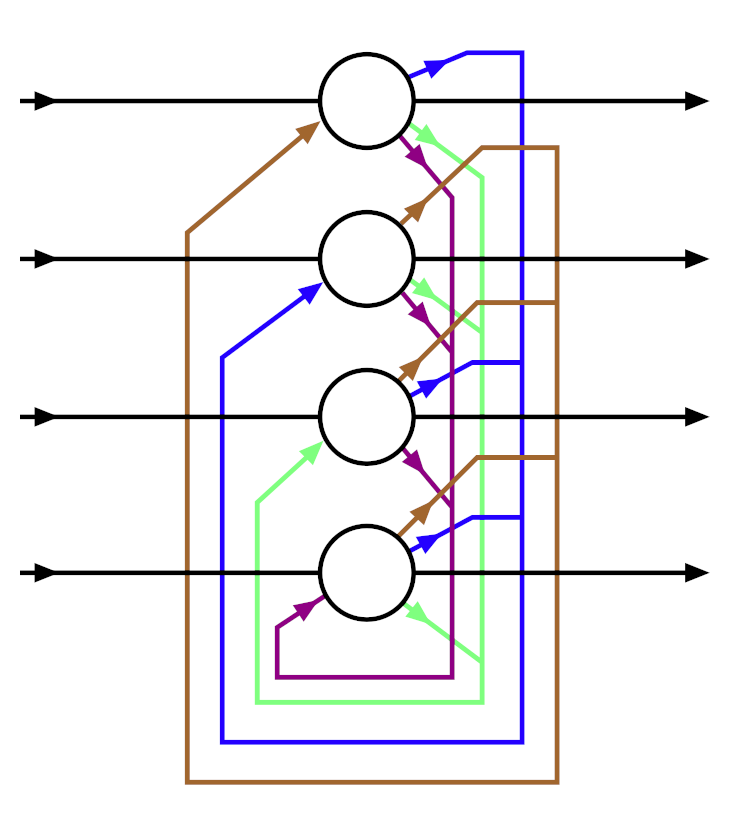
\includegraphics[width=0.95\linewidth]{../img/hopfieldnet.png}
	\caption{Circuit}
	\label{fig:netcircuit}
	\end{subfigure}
	\begin{subfigure}{0.4\textwidth}
	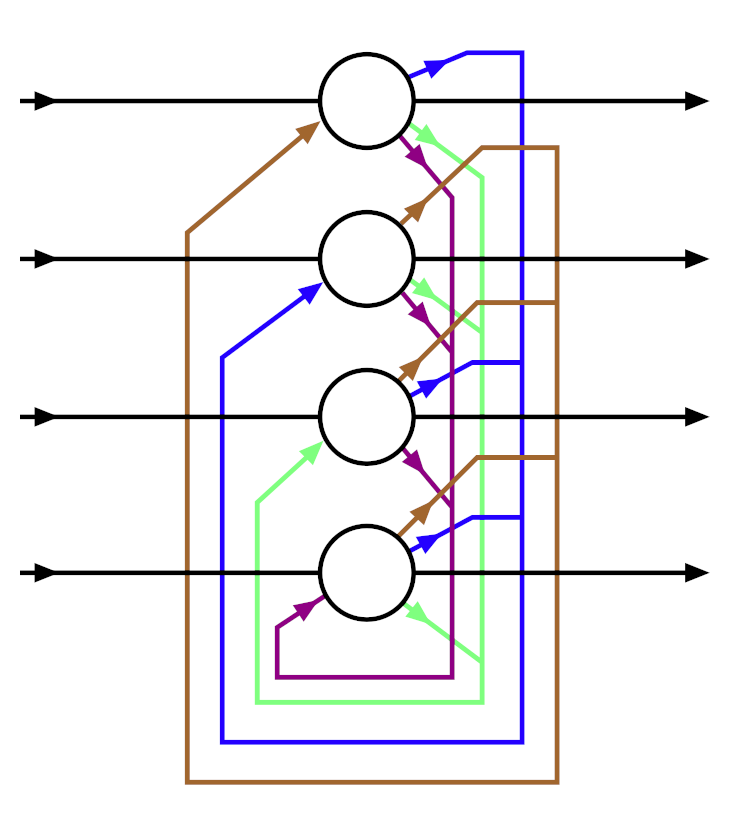
\includegraphics[width=0.95\linewidth]{../img/hopfieldnet.png}
	\caption{Graph}
	\label{fig:netgraph}
	\end{subfigure}
	\caption{Two equivalent diagrams of a Hopfield network of 4 nodes}
	\label{fig:net}
	\end{center}
	\end{figure}

	
	\begin{figure}
	\begin{center}
	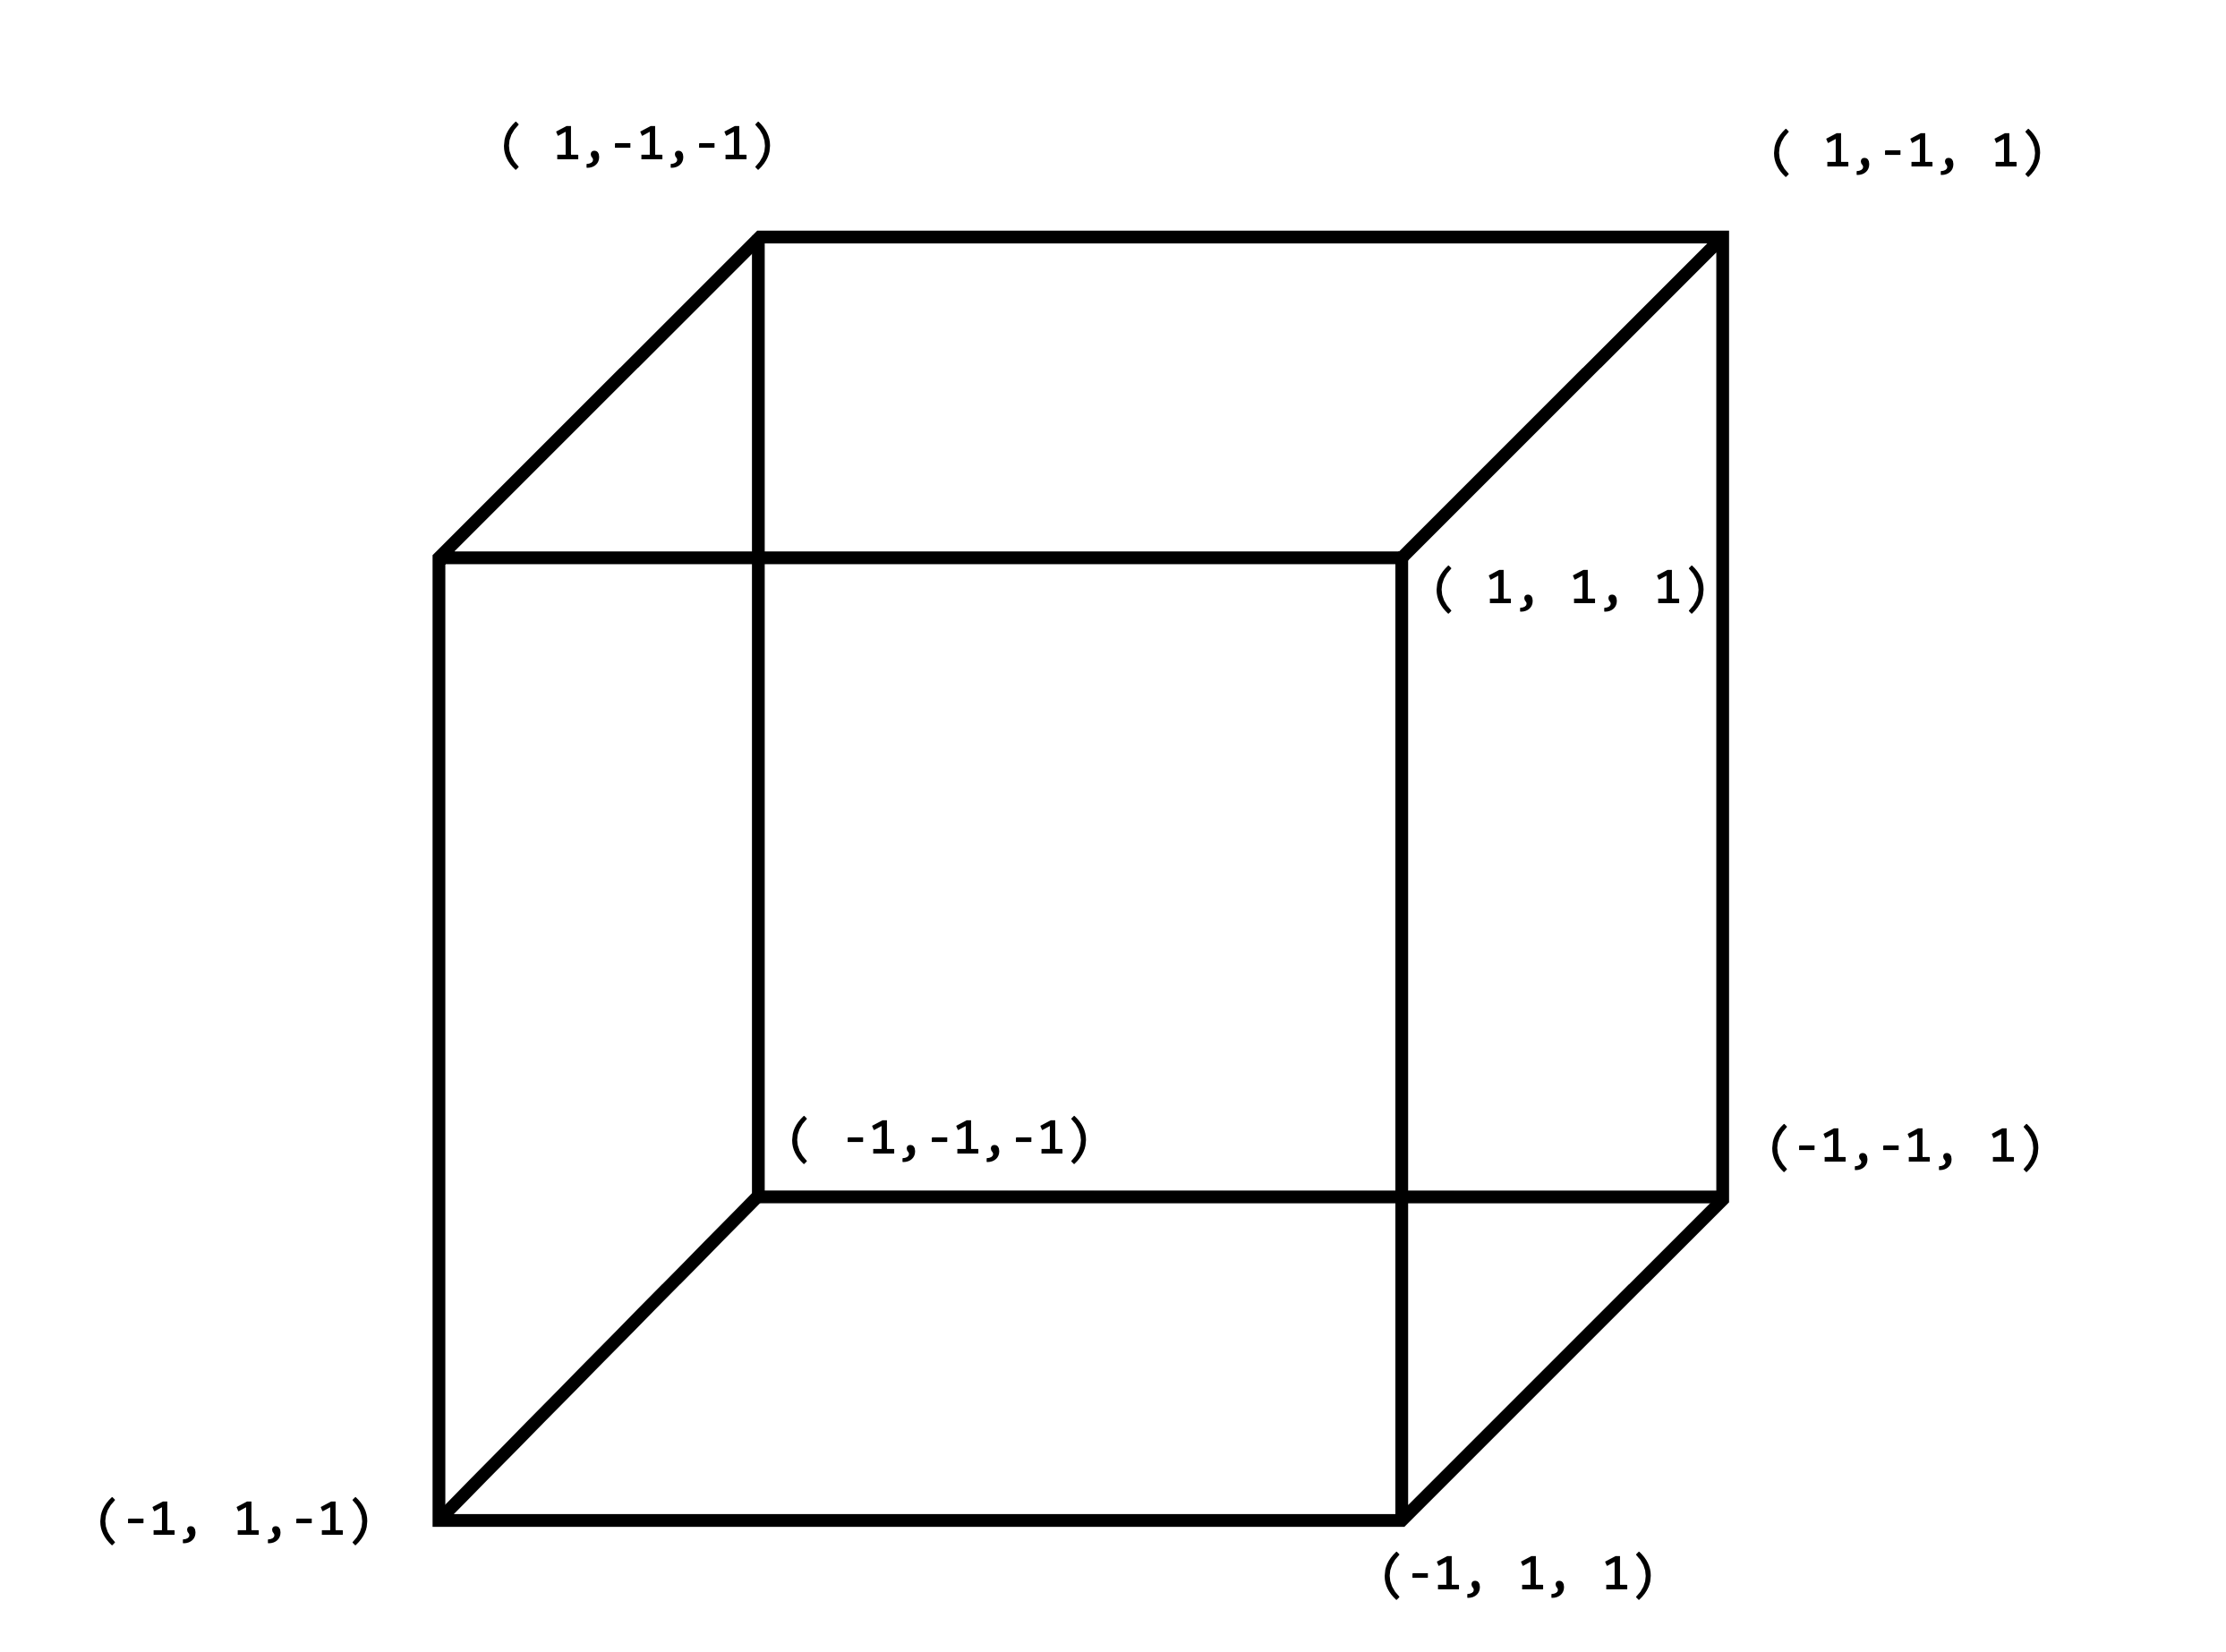
\includegraphics[width=0.35\textwidth]{../img/hypercube.png}
	\end{center}
	\caption{Unit hypercube representation of a three-dimensional vector}
	\label{fig:hypercube}
	\end{figure}		

	
	\begin{figure}
	\begin{center}
	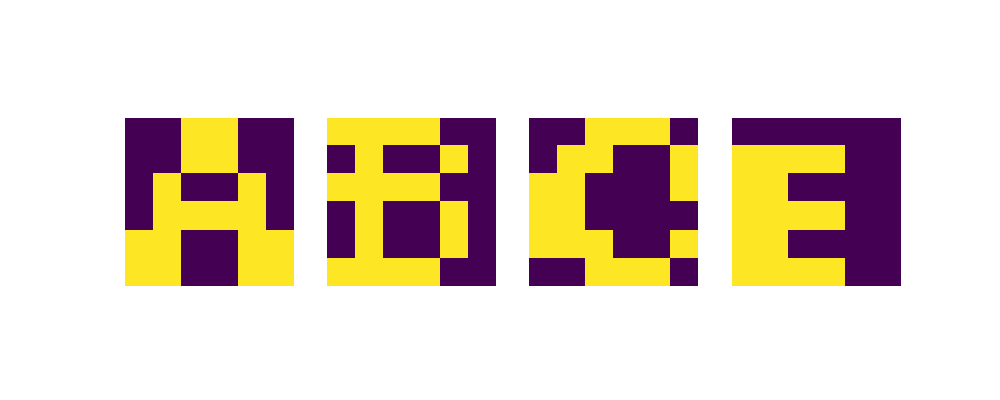
\includegraphics[width=1\textwidth]{../img/small_letters.png}
	\caption{Dataset of 6x6 letters}
	\label{fig:smallletters}
	\end{center}	
	\end{figure}


	\begin{figure}
	\begin{center}
	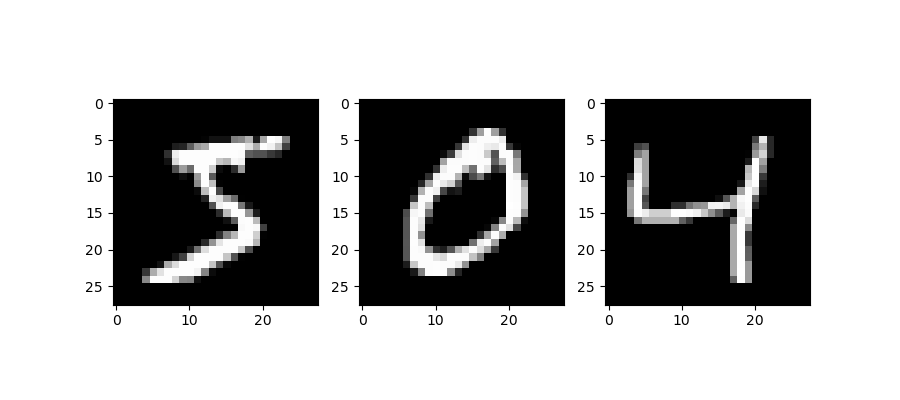
\includegraphics[width=0.8\textwidth]{../img/digits.png}
	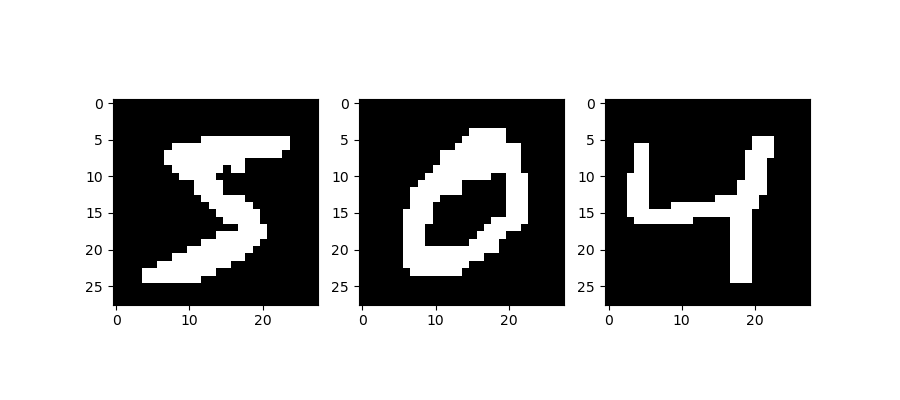
\includegraphics[width=0.8\textwidth]{../img/digits_shifted.png}
	\caption{MNIST dataset of 28x28 grayscale digits.\\ Original grayscale (top), shifted (bottom)}
	\end{center}	
	\label{fig:digits}
	\end{figure}
%
%	\begin{figure}
%	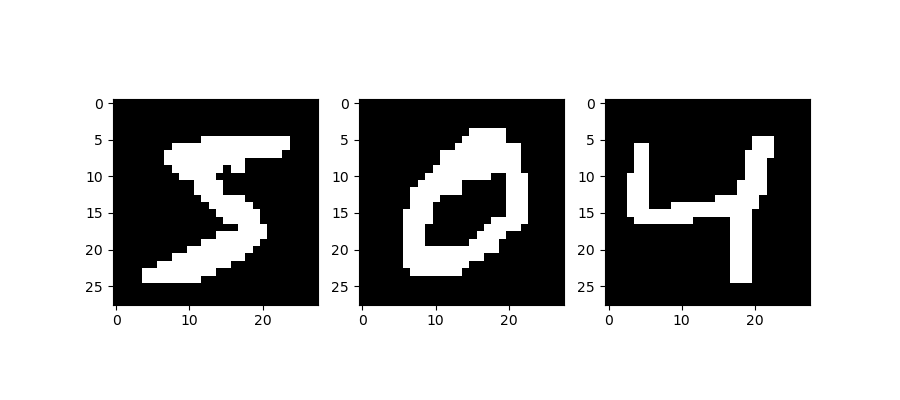
\includegraphics[scale=0.5]{../img/digits_shifted.png}	
%	\end{figure}	
%	
%	\begin{center}
%	\begin{figure}
%	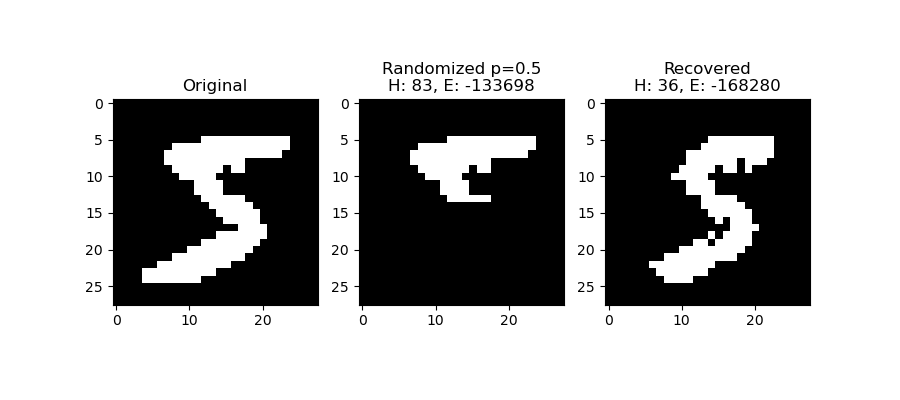
\includegraphics[scale=0.5]{../img/digits_result_good_covered.png}
%	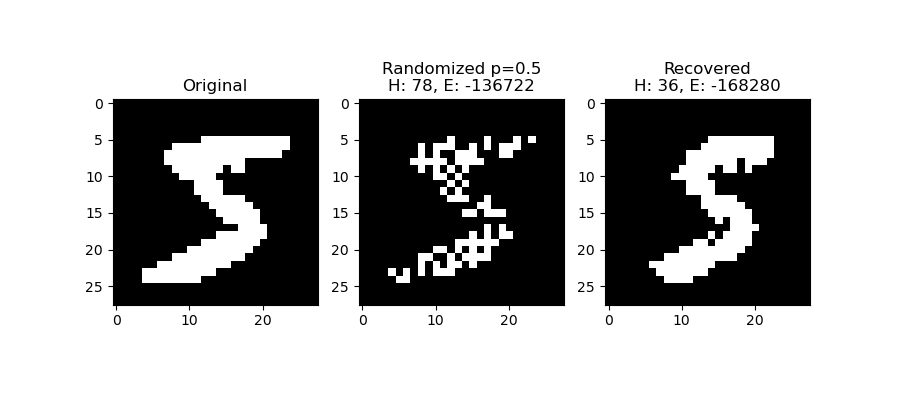
\includegraphics[scale=0.5]{../img/digits_result_good_random.png}	
%	\end{figure}
	
\end{document}
